% --------------------------------------------------------------------------------

\begin{exercise}

Sei $P_p:= \mathcal{L} \Bbraces{x^i y^j: i, j \geq 0 \land i+j \leq p}$ für $p \in \N$ der Raum der Polynome vom maximalen Grad $p$.

\begin{enumerate}[label = \textbf{\alph*)}]

  \item Geben Sie eine Basis von $P_0$ an.

  \item Zeigen Sie, dass die Funktionen

  \begin{align}
    \lambda_1(x, y) := 1-x-y,
    \quad
    \lambda_2(x, y) := x,
    \quad
    \lambda_3(x, y) := y
  \end{align}

  eine Basis des $P_1$ bilden.

  \item Zeigen Sie, dass die Funktionen $\lambda_1, \lambda_2, \lambda_3, \lambda_1 \lambda_2, \lambda_1 \lambda_3, \lambda_2\lambda_3$ eine Basis des $P_2$ bilden.

  \item Zeigen Sie, dass eine Basis des $P_p$ für $p \geq 3$ aus folgenden Funktionen gebildet werden kann:

  \begin{enumerate}[label = (\roman*)]
    \item $(x, y) \mapsto \lambda_j(x, y)$ mit $1 \leq j \leq 3$
    \item $(x, y) \mapsto p_{jk}(x, y)\lambda_j(x, y)\lambda_k(x, y)$ mit $1 \leq k < j \leq 3$ und
    \item $(x, y) \mapsto p_{123}(x, y) \prod_{j=1}^3 \lambda_j(x, y)$ und $p_{123} \in P_{p-3}$
  \end{enumerate}

  Die folgenden Einschränkungen der Polynome $p_{jk}$ sind dabei jeweils eindimensionale Polynome vom maximalen Grad $p-2: \xi \mapsto p_{12}(\xi, 0), \xi \mapsto p_{13}(0, \xi)$ und $\xi \mapsto p_{23}(\xi, 1-\xi)$.

  \item Erklären Sie anhand des Referenzdreiecks mit den Eckpunkten $(0, 0)$, $(1, 0)$ und $(0, 1)$ die Bedeutung dieser Aufgabe auf eine Erweiterung von Proposition $3.1$ auf Polynomräume höheren Grades.

\end{enumerate}

\end{exercise}

% --------------------------------------------------------------------------------

\begin{solution}

\begin{align*}
  \lambda_1(x, y) & = 1 - x - y \\
  \lambda_2(x, y) & = x \\
  \lambda_3(x, y) & = y \\
  (\lambda_1 \lambda_2)(x, y) & = x - x^2 - xy \\
  (\lambda_2 \lambda_3)(x, y) & = xy \\
  (\lambda_3 \lambda_1)(x, y) & = y - xy - y^2 \\
  (\lambda_1 \lambda_2 \lambda_3)(x, y) & = xy - x^2 y - x y^2
\end{align*}
Wir bezeichnen mit $B_p$ die kanonische Basis des $P_p$ und zeigen, dass
sich die gewünschten Basen durch eine Matrixtransformation der kanonischen Basis
darstellen lassen.
\begin{align*}
  B_p(x, y) := (1, x, y, x^2, xy, y^2, \dots, x^p, \dots, y^p)
\end{align*}

\begin{enumerate}[label = \textbf{\alph*)}]

  \item $\Lambda_0(x,y) := (1) = B_0(x,y)$
  \item

  \begin{align*}
    \Lambda_1
    :=
    \begin{pmatrix}
      \lambda_1 \\
      \lambda_2 \\
      \lambda_3
    \end{pmatrix}
  \end{align*}

  \begin{align*}
    \implies
    \underbrace
    {
      \begin{pmatrix}
        1 & -1 & -1 \\
          &  1 &    \\
          &    &  1
      \end{pmatrix}
    }_{
      =: T_1 \in \GL(3, \R)
    }
    B_1(x, y)
    =
    \Lambda_1(x, y)
  \end{align*}

  \item

  \begin{align*}
    \Lambda_2
    :=
    \begin{pmatrix}
      \Lambda_1 \\
      \lambda_1 \lambda_2 \\
      \lambda_2 \lambda_3 \\
      \lambda_3 \lambda_1
    \end{pmatrix}
  \end{align*}

  \begin{align*}
    \implies
    \underbrace
    {
      \pbraces
      {
        \begin{array}{ccc|ccc}
        1  &  -1   & -1   &    & & \\
          & 1 &    &    & & \\
          &     & 1   &    & & \\
          \hline
          & 1   &    & -1 & -1 & \\
          &     &    &    &  1 & \\
          &     &  1 & -1 &    & -1
        \end{array}
      }
    }_{
      =: T_2 \in \GL(6, \R)
    }
    B_2(x, y)
    =
    \Lambda_2(x, y)
  \end{align*}

  \item Wir definieren unsere Basis rekursiv.

  RA($p = 3$):

  \begin{align*}
    \Lambda_3(x, y)
    :=
    \begin{pmatrix}
      \Lambda_2(x, y) \\
      x \lambda_1(x, y) \lambda_2(x, y) \\
      x \lambda_2(x, y) \lambda_3(x, y) \\
      y \lambda_3(x, y) \lambda_1(x, y) \\
      x \lambda_3(x, y) \lambda_1(x, y)
    \end{pmatrix}
    =
    \begin{pmatrix}
      \Lambda_2 \\
      p_{12} \lambda_1 \lambda_2 \\
      p_{23} \lambda_2 \lambda_3 \\
      p_{31} \lambda_3 \lambda_1 \\
      \lambda_1 \lambda_2 \lambda_3
    \end{pmatrix}
    (x, y)
  \end{align*}

  $\Lambda_3$ ist linear unabhängig, weil $\Lambda_2$ es ist und jede Funktion $f$, ist zu $\id \cdot f$.
  Wir müssen die Transformationsmatrix also nicht einmal explizit hinschreiben. \\

  RS($p \mapsto p+1$):

  (i)-(iii) bedeuten hier, dass man $p_{12}$ mit $x$ und $p_{21}$ mit $y$ sowie $p_{23}, p_{123}$ entweder mit $x$ oder $y$ multiplizieren darf.
  Die Polynome werden dann (i)-(iii) im $p+1$ setting erfüllen.

  Seien $\Lambda_{p-1}$ und $\Lambda_p$ Basen von $P_p$ bzw. $P_{p-1} \subset P_p \subset P_{p+1}$.
  Wir ergänzen $\Lambda_p$ zu einer Basis $\Lambda_{p+1}$ von $P_{p+1}$, die (i)-(iii) für $p+1$ erfüllt.

  Die Elemente aus $\Lambda_p \setminus \Lambda_{p-1}$ (und $\Lambda_{p-1}$) haben folgende Form.

  \begin{align*}
    p_{12} \lambda_1 \lambda_2,
    \quad
    p_{23} \lambda_2 \lambda_3,
    \quad
    p_{31} \lambda_3 \lambda_1,
    \quad
    p_{123} \lambda_1 \lambda_2 \lambda_3,
    \quad
    (\text{und}~ \lambda_1, \lambda_2, \lambda_3)
  \end{align*}

  Polynome 1. und 3. Form multiplizieren wir mit $x$ bzw $y$;
  bei den anderen dürfen wir es uns jeweils aussuche, z.B. immer $x$.
  Wir erhalten $|\Lambda_p \setminus \Lambda_{p-1}| = p$ neue Polynome.
  Für das $(p+1)$-te Polynom nehmen wir die 2. oder 4. Form mal $y$.

  \begin{align*}
    \begin{Bmatrix}
      p_{12} \lambda_1 \lambda_2 \\
      p_{23} \lambda_2 \lambda_3 \\
      p_{31} \lambda_3 \lambda_1 \\
      p_{123} \lambda_1 \lambda_2 \lambda_3
    \end{Bmatrix}
    \mapsto
    \begin{Bmatrix}
      x \, p_{12} \lambda_1 \lambda_2 \\
      x \, p_{23} \lambda_2 \lambda_3 \\
      y \, p_{31} \lambda_3 \lambda_1 \\
      x \, p_{123} \lambda_1 \lambda_2 \lambda_3 \\
      y \, p_{123} \lambda_1 \lambda_2 \lambda_3
    \end{Bmatrix}
    \mapsto
    \begin{Bmatrix}
      x x \, p_{12} \lambda_1 \lambda_2 \\
      x x \, p_{23} \lambda_2 \lambda_3 \\
      y y \, p_{31} \lambda_3 \lambda_1 \\
      x x \, p_{123} \lambda_1 \lambda_2 \lambda_3 \\
      x y \, p_{123} \lambda_1 \lambda_2 \lambda_3 \\
      y y \, p_{123} \lambda_1 \lambda_2 \lambda_3
    \end{Bmatrix}
    \mapsto
    \begin{Bmatrix}
      x x x \, p_{12} \lambda_1 \lambda_2 \\
      x x x \, p_{23} \lambda_2 \lambda_3 \\
      y y y \, p_{31} \lambda_3 \lambda_1 \\
      x x x \, p_{123} \lambda_1 \lambda_2 \lambda_3 \\
      x x y \, p_{123} \lambda_1 \lambda_2 \lambda_3 \\
      x y y \, p_{123} \lambda_1 \lambda_2 \lambda_3 \\
      y y y \, p_{123} \lambda_1 \lambda_2 \lambda_3
    \end{Bmatrix}
    \mapsto \dots
  \end{align*}

  \item

  \begin{figure}[h!]
    \centering
    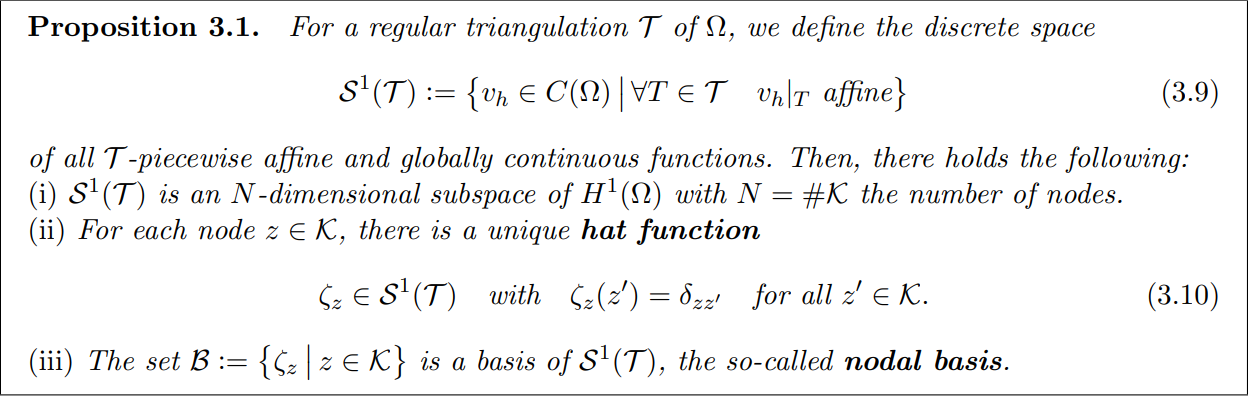
\includegraphics
    [width = 0.75 \textwidth]
    {NumPDEs/NumPDEs - Proposition 3.1.png}
    \caption{\cite{NumPDEs}}
  \end{figure}

  \begin{comment}

  Ganz Allgemein:

  Sei $B$ eine Polynombasis von $P_p$, und $n := \dim P_p = |B|$.
  Seien $(x_1, y_1), \dots, (x_n, y_n) \in \K^2$ paarweise verschiedene Interpolations-Knoten und $p(x_1, y_1), \dots, p(x_n, y_n) \in \K$ Interpolations-Werte.
  Durch ein lineares Gleichungssystem mit Vandermonde-Matrix bzgl. $B$ und $(x_1, y_1), \dots, (x_n, y_n)$ als linke Seite und $(p(x_1, y_1), \dots, p(x_n, y_n))^T$ als rechte Seite, können wir die Koeffizienten eines eindeutigen Polynoms $p \in P_p$ finden, dass an den Interpolations-Knoten die gewünschten Interpolations-Werte annimmt. \\

  In unserem Fall:

  Wenn wir in Proposition 3.1 von Ordnung $p$ nach $p + 1$ gehen, dann müssen wir $p + 1$ Interpolations-Knoten (aus dem Dreieck) und -Werte hinzufügen.

  Wir wollen, dass unser (durch die lokale Interpolation auf den Dreiecken zusammengesetzter) Spline stetig ist.
  Außerhalb der Kanten ist das immer der Fall.
  Auf den Kanten müssten die angrenzenden Interpolations-Polynome übereinstimmen.

  Das erzielen wir, indem wir beim Ordnungs-Übergang zu jeder Kante genau einen Interpolations-Knoten hinzufügen.
  (Den Rest packen wir ins Innere der Dreiecke.)
  Für jede Kante sind die darauf eingeschränkten Interpolations-Polynome eindeutig bestimmt.
  Insbesondere stimmen angrenzende Polynome darauf überein.

  \end{comment}

  Wir können mit der Basis aus \textbf{d)} \Quote{verallgemeinerte Hutfunktionen} bauen, d.h. eine Basis des Spline-Raums der Ordnung $p$ mit Funktionen, die Definitionsbereich im Gebiet $\Omega \subset \R^2$ haben.
  Diese Basisfunktionen sind, so wie die normalen Hutfunktionen, stetig und haben lokalen $\supp$.

  Das ist klar für Basisfunktionen, die sich aus Polynomen vom Typ (i) zusammensetzen, weil das ja gerade die normalen Hutfunktionen sind.
  Für die vom Typ (iii) ist das auch klar, weil die am Rand des jeweiligen Dreiecks (d.h. auf allen Kanten) verschwinden.
  Basisfunktionen bestehend aus Polynomen vom Typ (ii) verschwinden nur auf $2$ Kanten.

  Sie sind aber dennoch stetig und besitzen lokalen $\supp$.
  Betrachten wir dazu zwei Dreiecke $T_1, T_2 \in \mathcal{T}$ mit gemeinsamer Kante $E$.
  Seien $b_1$ und $b_2$ (Basis-Polynome) die Teile einer verallgemeinerten Hutfunktionen $b$ vom Typ (ii) auf den Dreiecken $T_1$ bzw. $T_2$, die auf $E$ nicht verschwinden.
  Sei $(x, y) \in E$.
  Für die Stetigkeit soll gelten, dass $b_1(x, y) = b_2(x, y)$.
  Nachdem $b_1$ und $b_2$ durch Transformation von $b_0$, dem zugehörigen Basis-Polynom auf dem Referenzdreieck $T_\mathrm{ref}$, auf $T_1$ bzw. $T_2$ gebildet werden, ist dies der Fall.
  (Die Transformation interessiert sich ja nicht für konkrete Dreiecke, sondern nur für den Punkt, wohin man transformieren will.)

\end{enumerate}

\end{solution}

% --------------------------------------------------------------------------------
